\section{Domain-Independent Methods}
\label{sec:domain-independent-methods}

\textbf{Domain-independent methods} use a symbolic model of the domain and problem to solve tasks. Unlike domain-specific algorithms, they employ generic search algorithms that work across different problem domains.

\subsection{Problem Representation}
\label{subsec:problem-representation}

For example, in the Towers of Hanoi problem, we would define the problem in general terms as follows:

\begin{figure}[H]
    \centering
    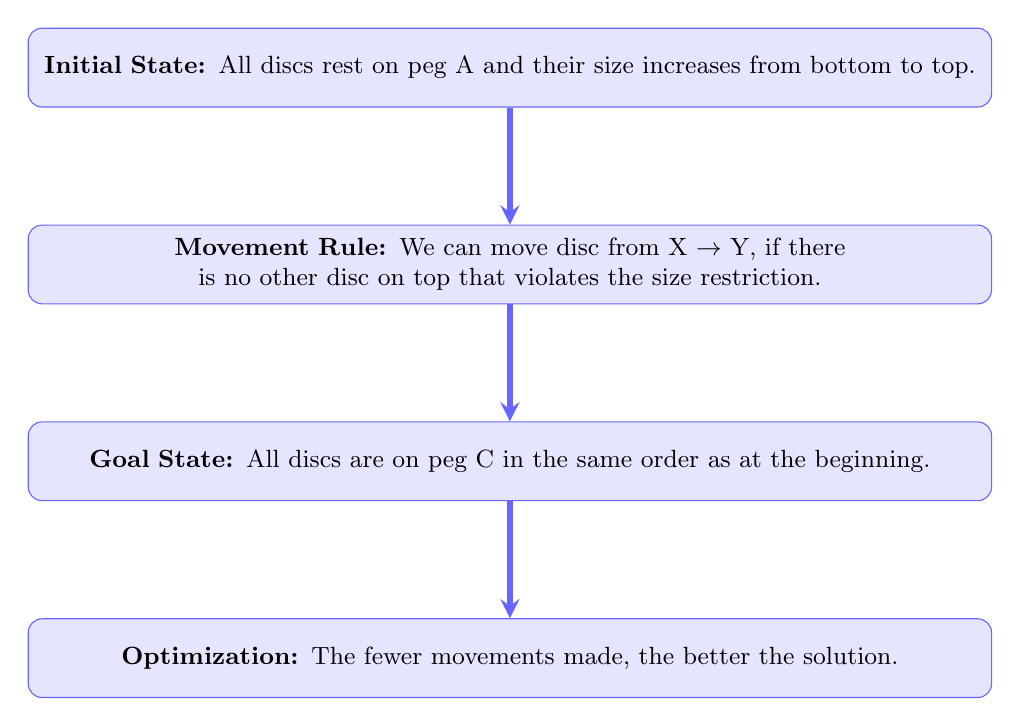
\begin{tikzpicture}[
        box/.style={rectangle, rounded corners=5pt, draw=blue!60, fill=blue!10, text width=12cm, minimum height=1cm, align=center, font=\small},
        arrow/.style={->, >=stealth, blue!60, line width=2pt}
    ]
        % Boxes
        \node[box] (initial) at (0,0) {\textbf{Initial State:} All discs rest on peg A and their size increases from bottom to top.};
        
        \node[box] (rule) at (0,-2.5) {\textbf{Movement Rule:} We can move disc from X $\rightarrow$ Y, if there is no other disc on top that violates the size restriction.};
        
        \node[box] (goal) at (0,-5) {\textbf{Goal State:} All discs are on peg C in the same order as at the beginning.};
        
        \node[box] (optimization) at (0,-7.5) {\textbf{Optimization:} The fewer movements made, the better the solution.};
        
        % Arrows
        \draw[arrow] (initial.south) -- (rule.north);
        \draw[arrow] (rule.south) -- (goal.north);
        \draw[arrow] (goal.south) -- (optimization.north);
    \end{tikzpicture}
    \caption{Symbolic representation of the Towers of Hanoi problem using domain-independent methods.}
    \label{fig:hanoi-problem-definition}
\end{figure}

\subsection{Advantages}
\label{subsec:domain-independent-advantages}

To solve problems, this method employs a \textbf{generic search algorithm}, representing the domain and problem through the symbolic model. This approach offers several advantages:

\begin{itemize}
    \item \textbf{Greater flexibility}: We do not need to know the solution beforehand. The search algorithm explores the solution space automatically.
    
    \item \textbf{Easy extensibility}: It is straightforward to add new features or constraints to the problem by modifying the symbolic model, without changing the search algorithm itself.
    
    \item \textbf{Reusability}: The same generic search algorithm can be applied to different problem domains by simply changing the symbolic representation.
\end{itemize}
